\documentclass{article} % For LaTeX2e
\usepackage{iclr2025,times}

\usepackage{hyperref}
\usepackage{url}
\usepackage{graphicx}
\usepackage{subfigure}
\usepackage{booktabs}
\usepackage{amsmath}
\usepackage{amssymb}
\usepackage{mathtools}
\usepackage[capitalize,noabbrev]{cleveref}

\graphicspath{{../figures/}} % To reference your generated figures, name the PNGs directly. DO NOT CHANGE THIS.

\begin{filecontents}{references.bib}
@book{goodfellow2016deep,
  title={Deep learning},
  author={Goodfellow, Ian and Bengio, Yoshua and Courville, Aaron and Bengio, Yoshua},
  volume={1},
  year={2016},
  publisher={MIT Press}
}
\end{filecontents}

\title{
Learning Congestion Maps from Path Planning Conflicts:\\
Structured Signals, Limited Gains for Decoupled Scheduling
}

\author{Anonymous}

%\iclrfinalcopy
\begin{document}

\maketitle

\begin{abstract}
Decoupled multi-agent scheduling is attractive because it preserves modularity: tasks are assigned first and path planning is delegated to a downstream solver. Its main weakness is that the allocator is blind to congestion, so assignments that look cheap geometrically can create avoidable bottlenecks. We studied Conflict Memory Allocation (CMA), a lightweight feedback loop that aggregates planner-reported conflicts into a spatial memory map and reuses that map as a soft penalty during future assignment. The retained artifact supports only part of the original hypothesis. The learned conflict memory is clearly non-uniform: the final map is sparse, with a few persistent hotspots that align with repeated bottleneck regions. However, these structured signals translated into little overall benefit. In the available evaluation, the best logged penalty weight was $0.5$, the corresponding labeled final improvement was only $0.0123$, and the logged improvement-ratio values were almost always near zero with one substantial negative outlier near $-0.2$. The main lesson is that learning where conflicts happen is easier than turning that knowledge into a decision signal strong enough to improve a decoupled allocator.
\end{abstract}

\section{Introduction}
\label{sec:intro}

Task allocation followed by path planning remains a practical default in multi-agent systems because the pipeline is simple, modular, and scalable. The downside is equally familiar: an assignment that appears short when each agent is considered independently can funnel many agents through the same aisle, doorway, or pickup region, leaving the path planner to absorb the damage. This motivates a simple question: can the planner's own conflicts be recycled as feedback for later allocations?

Our starting hypothesis was optimistic. If path-planning conflicts reflect stable features of the environment, then a lightweight congestion prior might recover some of the benefit of coupling without paying the cost of joint optimization. This is a small representation-learning problem: repeated local events are compressed into a reusable bias for future decisions \citep{goodfellow2016deep}. We therefore implemented Conflict Memory Allocation (CMA), a histogram-based memory that stores where conflicts happen and adds a soft penalty to assignments whose estimated routes traverse those locations.

The pilot logs only partially support this idea. The positive result is that conflict memory is \emph{learnable}: the final map is highly structured, sparse, and dominated by a few repeatable hotspots. The negative result is that this structure does not reliably improve scheduling. Across the available evaluation traces, the logged improvement-ratio values are visually concentrated at zero, the artifact's best-tuned run reports only a tiny aggregate gain, and one instance shows a clear regression. For real deployments, this is a useful failure case: detecting bottlenecks is not enough if the learned signal is too weak or too poorly aligned with the optimizer that is supposed to use it. We emphasize that the retained artifact supports a cautionary empirical claim, not a universal impossibility result.

\section{Related Work}
\label{sec:related}

Our study sits between strict decoupling, where assignment and planning are solved separately, and tighter integration, where downstream planning information influences upstream decisions. CMA tries to keep the modularity of the former while borrowing a small amount of feedback from the latter through learned cost shaping. In that sense, it follows the broader machine-learning view that a useful representation is one that changes a downstream decision rule rather than merely describing the data \citep{goodfellow2016deep}. The negative result here is exactly a failure of that last step: the learned conflict representation is visible and structured, but it is not strong enough to induce robust assignment changes. This framing is also why the result is relevant to an ICBINB-style workshop. The failure is not that the signal is random; the failure is that a plausible, interpretable, and apparently learnable signal still does not yield meaningful end-task improvement when inserted into a decoupled pipeline.

\section{Method}
\label{sec:method}

We consider a standard decoupled pipeline. A task allocator first chooses agent-to-task assignments using a baseline cost $c_0(a,t)$, typically derived from geometric distance or single-agent travel time. A path planner then computes collision-free routes. Planner conflicts are informative because they expose where the decoupled choice created competition for space and time.

CMA summarizes those conflicts in a reusable grid memory $M \in \mathbb{R}_{\ge 0}^{H \times W}$. After solving instance $k$, observed conflicts are projected into a grid histogram $C_k$, and the memory is updated by an exponential moving average,
\[
M_{k+1} = \beta M_k + (1-\beta) C_k,
\]
where $\beta$ controls forgetting. CMA does not change the downstream planner. Instead, it perturbs only the assignment cost,
\[
\tilde c(a,t) = c_0(a,t) + \lambda \sum_{v \in \hat P(a,t)} M(v),
\]
where $\hat P(a,t)$ is a single-agent shortest-path surrogate and $\lambda$ is a penalty weight. This design is deliberately lightweight, but it also exposes the core risk: a correct memory may still fail to change the chosen assignment if the surrogate path is a poor proxy for the final joint plan or if the added penalty is small relative to variation in $c_0(a,t)$.

\section{Experiments}
\label{sec:experiments}

The retained artifact is limited, and we report it conservatively. The provided \texttt{BASELINE\_SUMMARY} and \texttt{RESEARCH\_SUMMARY} JSON objects are empty, so every quantitative claim below comes directly from logged visualizations rather than recomputed aggregate statistics. We therefore keep only one main-text figure: a compact diagnostic that captures the paper's central empirical contrast. Other exported images were excluded from the scientific argument because their semantics are too weakly labeled to support reliable captions; we list those files in the appendix rather than treating them as evidence.

\begin{figure}[t]
\centering
\subfigure[Final conflict memory.]{
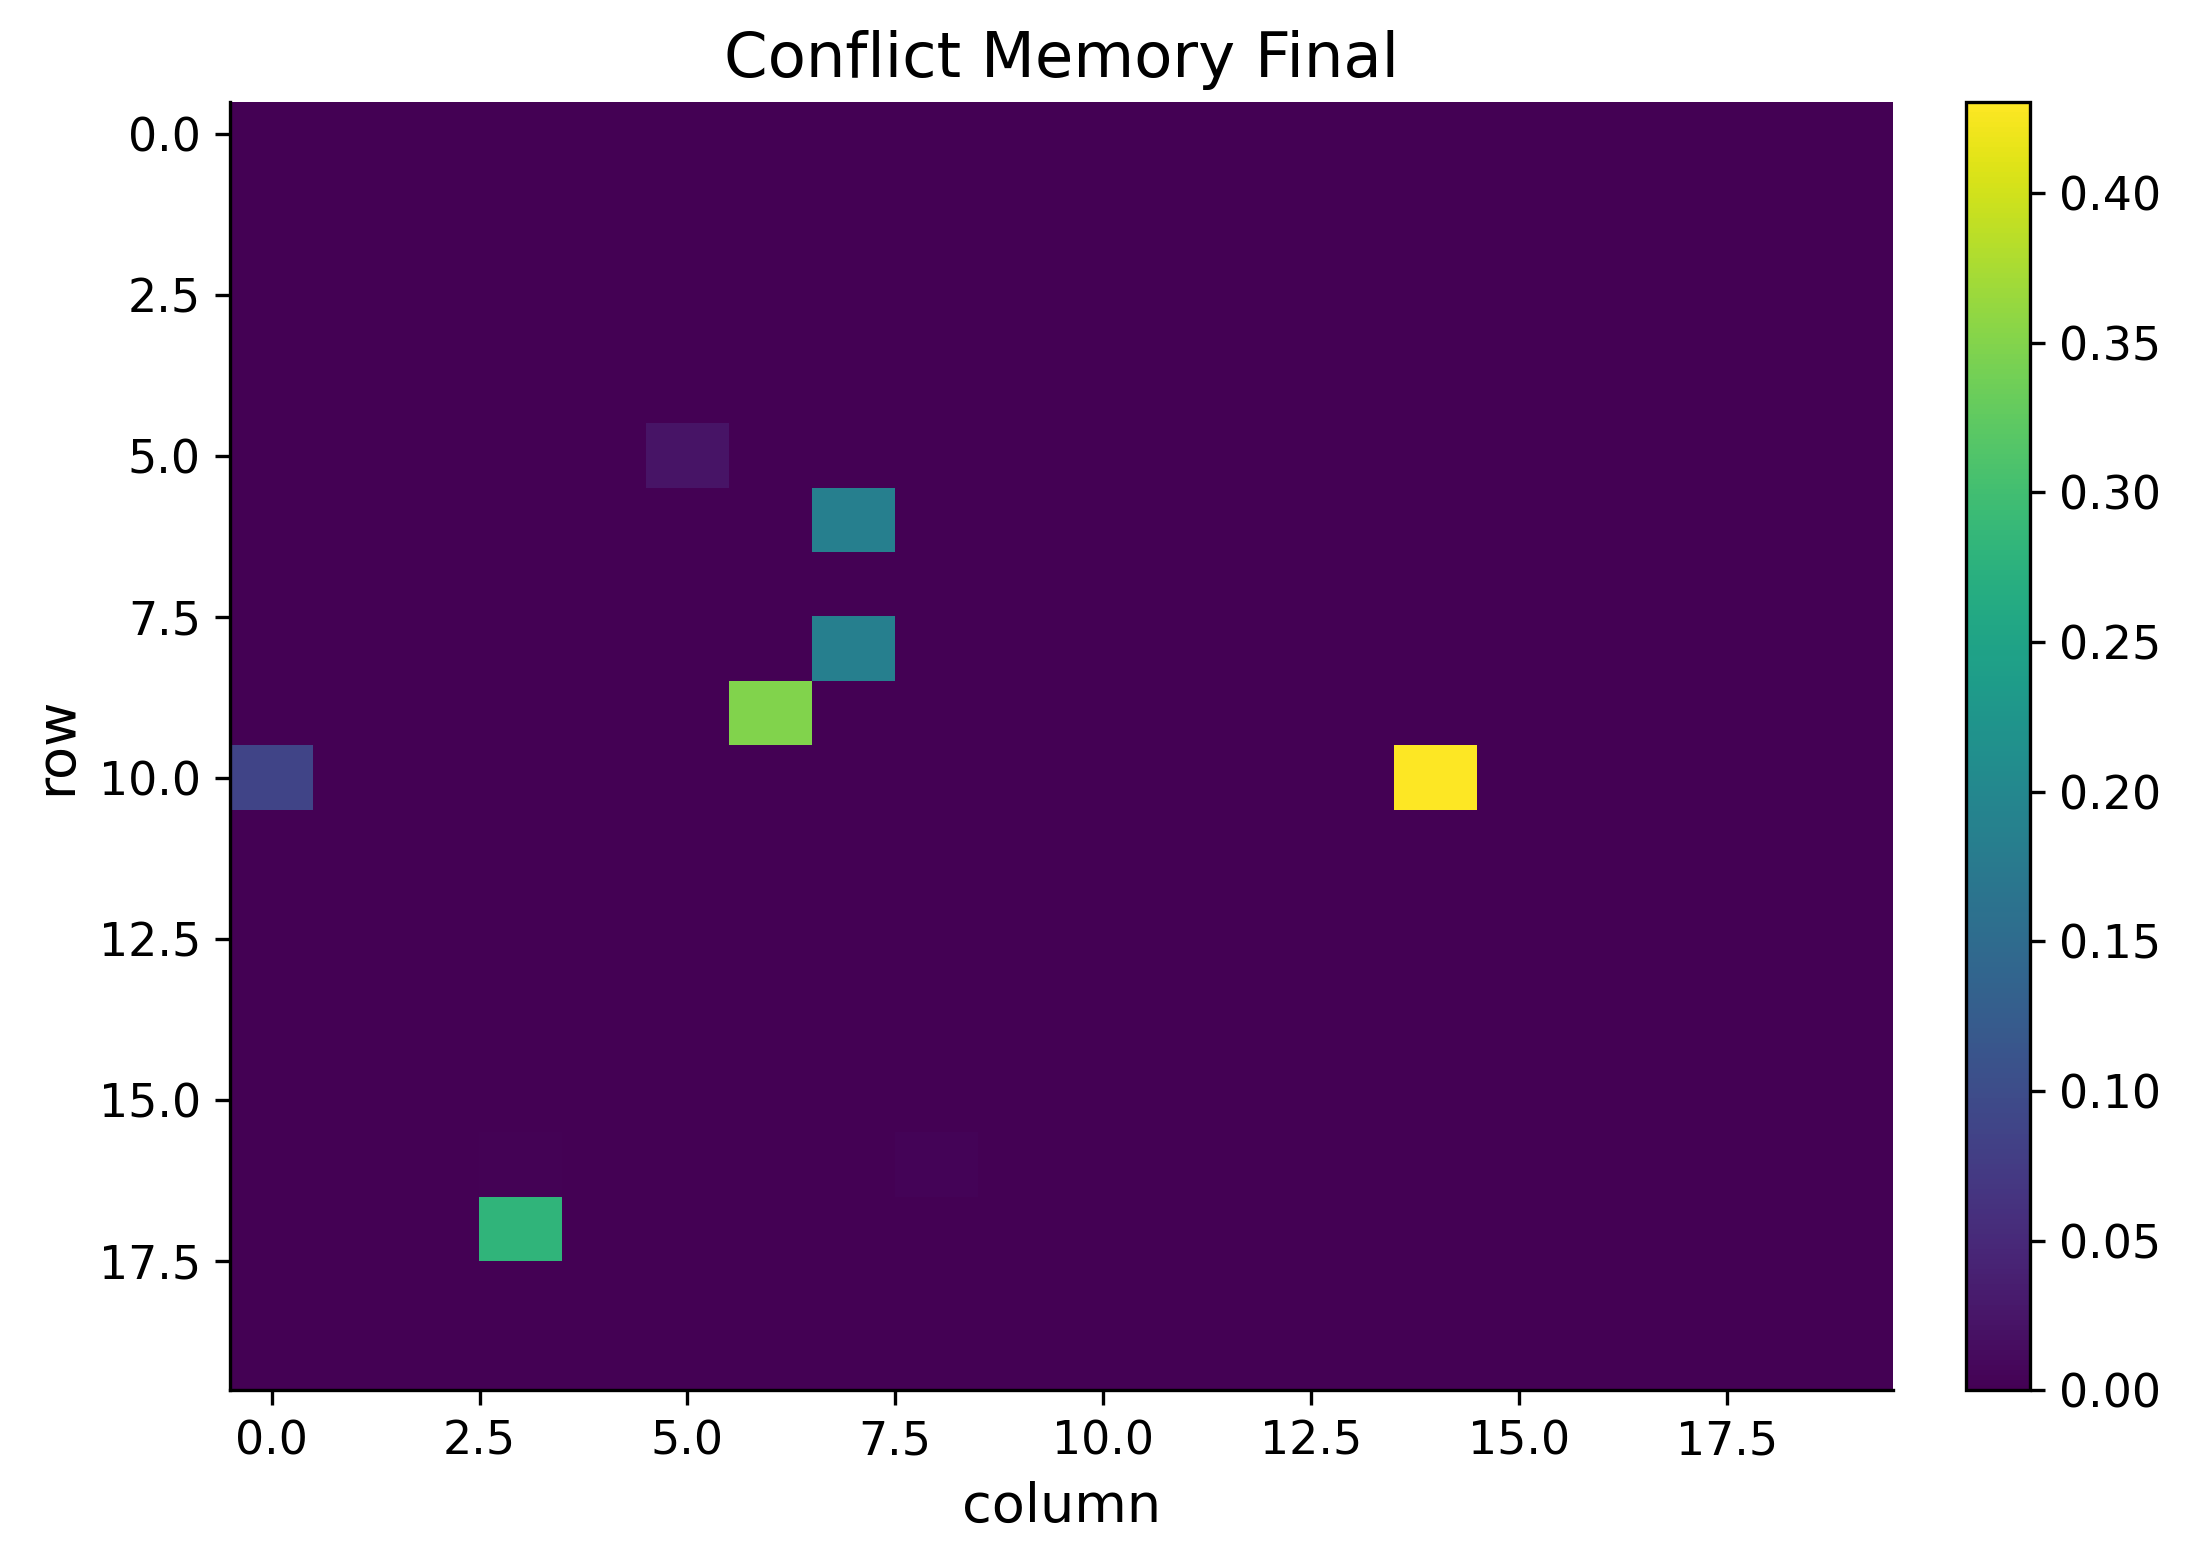
\includegraphics[width=0.46\textwidth]{conflict_memory_final.png}
\label{fig:memory_only}
}
\hfill
\subfigure[Improvement-ratio values by instance index.]{
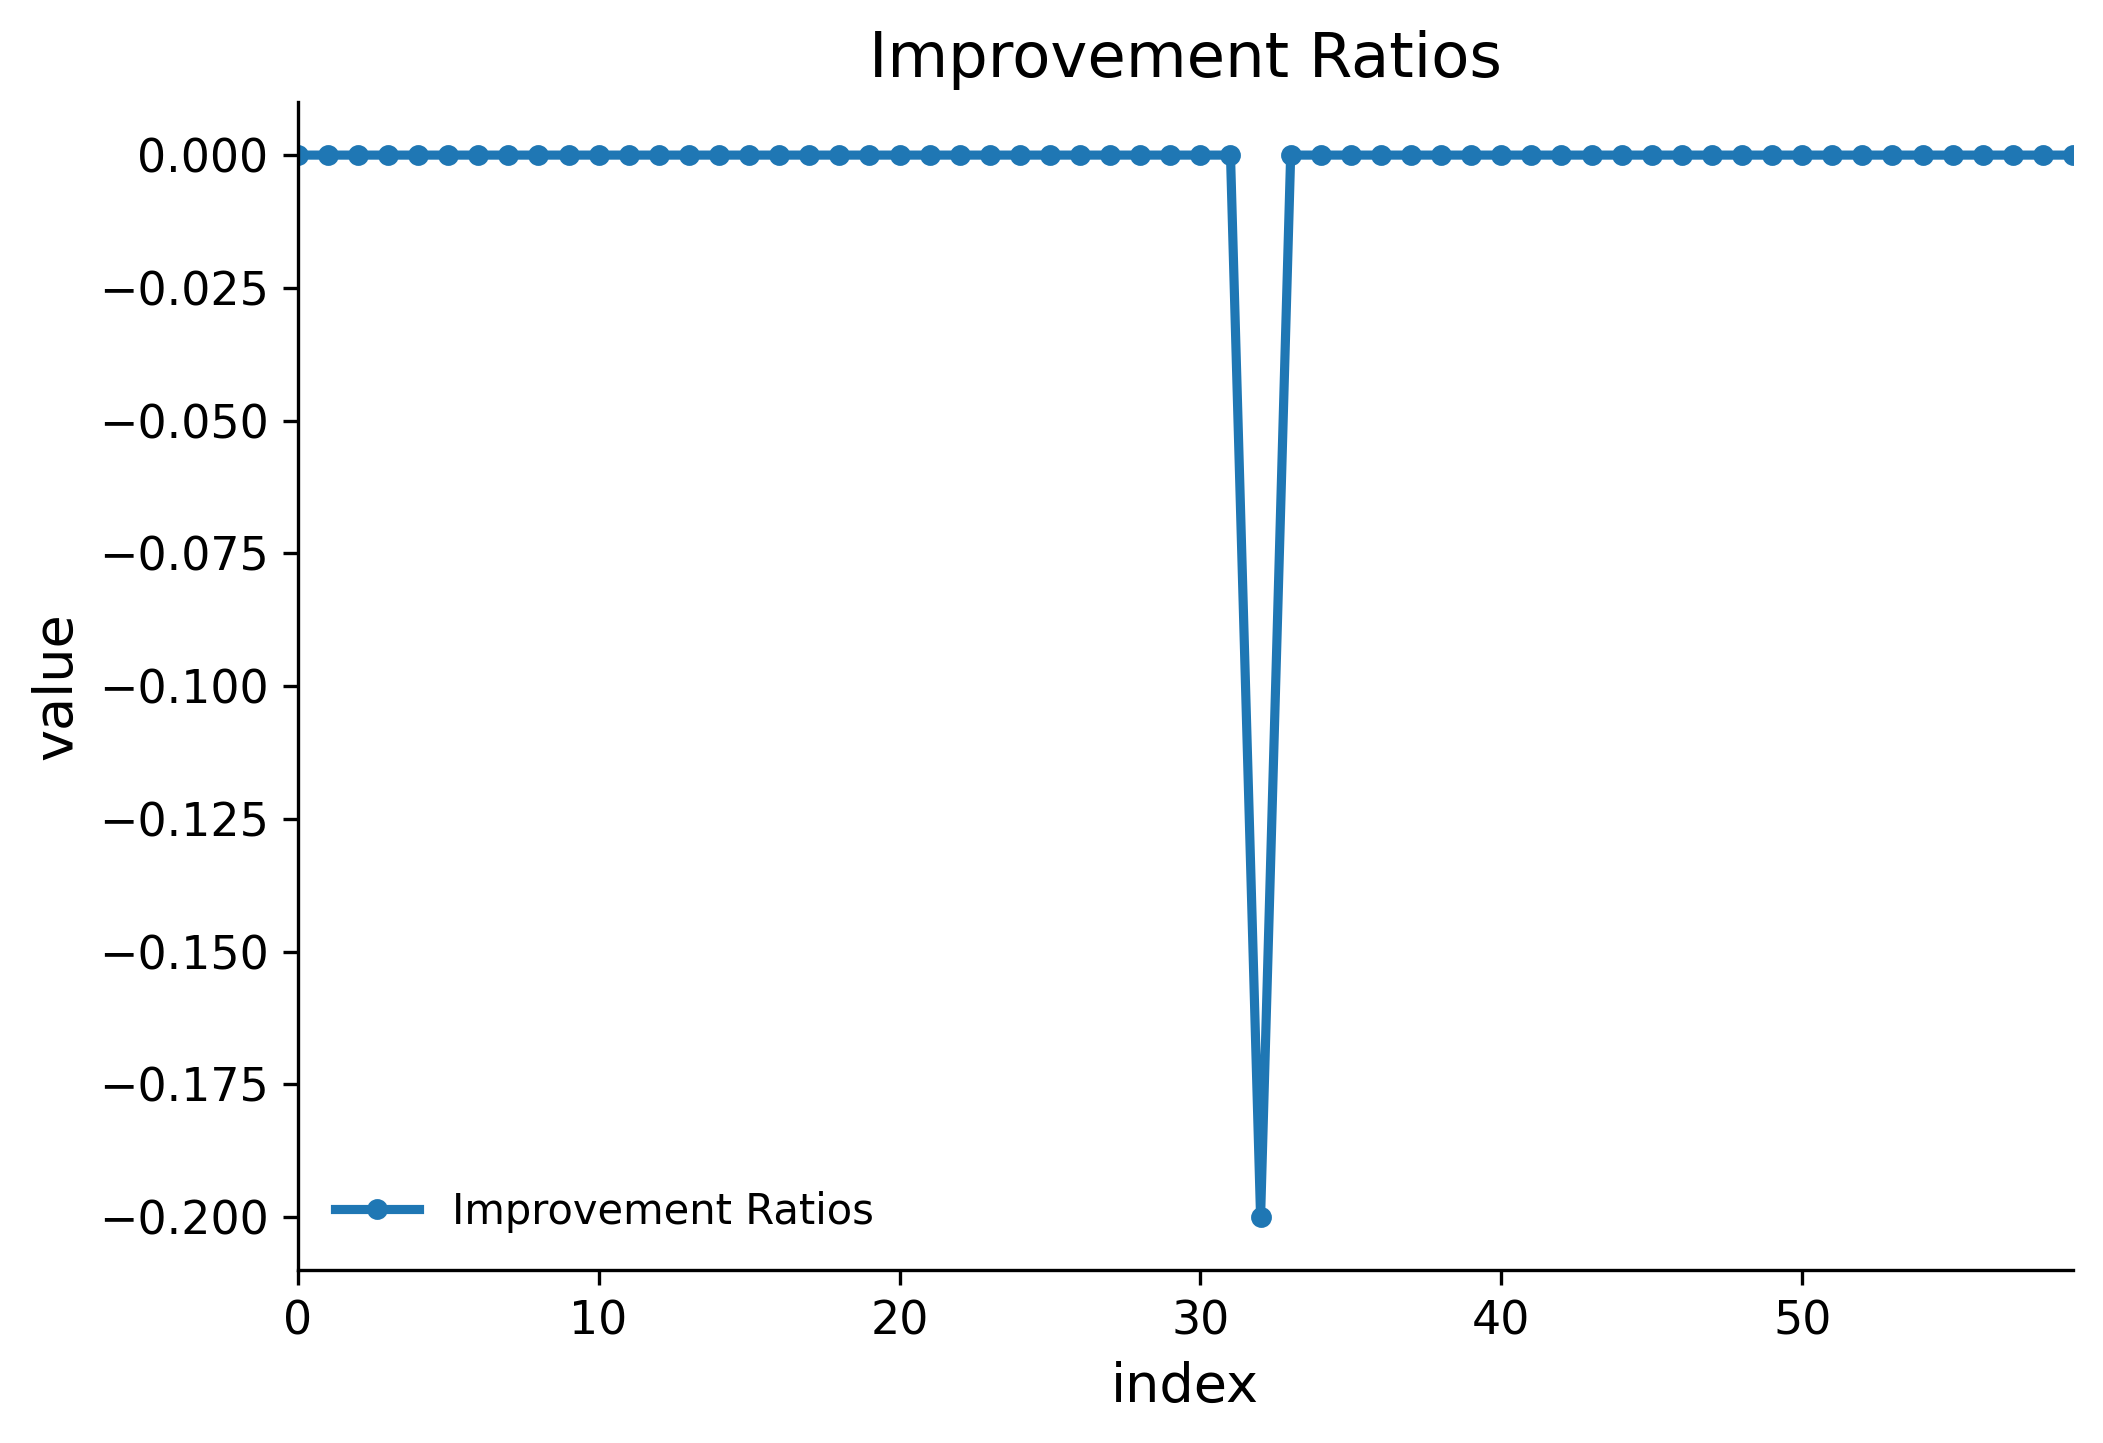
\includegraphics[width=0.46\textwidth]{improvement_ratios.png}
\label{fig:ratios_only}
}
\caption{Single-run diagnostic. (a) Final $20 \times 20$ conflict-memory map. Activation is sparse and concentrated in one dominant hotspot with a few weaker secondary cells. (b) Logged improvement-ratio values by instance index. Most values are at or extremely near zero, with one harmful outlier near $-0.2$. Together, the panels show that CMA learned stable spatial structure but rarely converted it into better outcomes.}
\label{fig:main_results}
\end{figure}

\begin{table}[t]
\centering
\small
\caption{Main empirical takeaways directly supported by the retained artifact.}
\label{tab:takeaways}
\begin{tabular}{p{0.24\linewidth}p{0.25\linewidth}p{0.35\linewidth}}
\toprule
Evidence source & Observation & Interpretation \\
\midrule
Tuning log & Best penalty weight $0.5$; labeled final improvement $0.0123$ & Even the best recovered setting yields only a very small aggregate gain. \\
Conflict-memory heatmap & Sparse map with one dominant hotspot and a few weaker cells & CMA learns persistent spatial structure rather than staying uniform. \\
Improvement-ratio plot & Most values lie near zero; one visible negative outlier near $-0.2$ & Benefits are inconsistent and occasional regressions are possible. \\
\bottomrule
\end{tabular}
\end{table}

Two exact scalars survive from the tuning logs: the best penalty weight was $\lambda=0.5$, and the corresponding labeled final improvement was only $0.0123$. Beyond those anchors, \Cref{fig:main_results} and \Cref{tab:takeaways} should be read diagnostically rather than statistically. The horizontal axis in \Cref{fig:ratios_only} is just an instance index, not training time, and the empty summary files prevent confidence intervals, seed-level aggregation, or significance tests.

The scientific value of \Cref{fig:memory_only} is that it rules out a trivial failure mode. CMA did not fail because the memory remained flat. The learned map is visibly sparse and low-entropy: most cells carry negligible weight, while a small number of locations dominate the penalty. That pattern is exactly what one would expect if the environment contains recurring chokepoints. At the same time, the concentration is so sharp that the learned prior may have limited leverage. If many candidate assignments traverse the same unavoidable hotspot, then a correct memory still produces nearly identical penalties for the options the allocator is comparing, leaving the ranking mostly unchanged.

\Cref{fig:ratios_only} shows the complementary failure. The downstream metric is almost zero-inflated: for most indexed instances, the improvement ratio is visually indistinguishable from zero. This suggests that CMA usually behaves as a weak perturbation rather than a decisive intervention. A useful way to interpret the negative outlier is not merely that CMA ``sometimes hurts,'' but that historical conflict memory can redirect traffic toward a different bottleneck without reducing the true joint critical path. In other words, a map of where conflicts used to occur is not yet a counterfactual model of which reassignment will reduce final makespan on the current instance.

From a deployment perspective, the tuning result is mildly informative rather than purely null. A best weight of $0.5$ indicates that the method was not disabled by a degenerate choice of $\lambda=0$. The more interesting failure is that nonzero use of the learned memory still does not create a strong enough change in assignment rankings to matter consistently downstream.

Taken together, the figure and table point to a specific interface mismatch. CMA learns a \emph{spatial} summary, but the downstream objective depends on \emph{spatiotemporal} multi-agent interactions. The assignment penalty is computed on a single-agent surrogate route, whereas the planner's actual collisions depend on simultaneous occupancy, route coupling, and local timing. Under that mismatch, the memory can be accurate as a descriptive statistic and still be weak as an optimization signal. This interpretation is consistent with the tiny best logged gain: whatever useful congestion information CMA captures is too weak, too local, or too stale to robustly alter the bottleneck that determines makespan.

\section{Conclusion}
\label{sec:conclusion}

This pilot study supports only half of the original CMA story. Path-planning conflicts do contain stable, spatially structured information, and a simple histogram memory recovers that structure cleanly. But in the retained experiments, feeding this memory back into assignment produced little measurable benefit: the best logged setting barely improved the aggregate metric, the per-instance values were almost always near zero, and one outlier showed that the feedback can hurt. The practical lesson is simple: before investing in learned congestion priors for decoupled scheduling, verify not only that the signal is learnable, but also that it is aligned strongly enough with the allocator to change decisions in the right direction. A promising next step is not merely to smooth or enlarge the memory, but to redesign the feedback signal so that it better reflects timing-sensitive interactions rather than static occupancy alone.

\bibliography{references}
\bibliographystyle{iclr2025}

\appendix
\section{Supplementary Material}
\label{sec:appendix}

\subsection{Figure-Selection Policy}

We were intentionally aggressive about figure selection. Only the paired diagnostic in \Cref{fig:main_results} remains in the main text because it directly supports the paper's central claim: CMA learns a structured memory, yet that structure rarely translates into better outcomes. We did \emph{not} move the other exported images into the appendix as figures, because the retained artifact does not provide enough context to caption them rigorously. Instead, we document them as unused exports below. This is a deliberate scientific choice: weakly labeled dashboards are better omitted than over-interpreted.

\subsection{Reproducibility Boundaries of the Retained Artifact}

The machine-readable \texttt{BASELINE\_SUMMARY} and \texttt{RESEARCH\_SUMMARY} objects were empty. As a result, the paper intentionally avoids claims about statistical significance, exact benchmark names, or seed-aggregated performance. The only exact scalar values recoverable from the artifact were the best penalty weight $0.5$ and the labeled final improvement $0.0123$.

\subsection{Recoverable Experimental Configuration}

Not every experimental detail survived in machine-readable form, but some configuration information can still be recovered from the artifact itself. \Cref{tab:recoverable_config} separates values that were directly logged from values that can only be inferred visually. We intentionally do not guess missing hyperparameters such as the memory decay factor $\beta$, benchmark identity, or seed count.

\begin{table}[h]
\centering
\small
\caption{Configuration details recoverable from the retained artifact.}
\label{tab:recoverable_config}
\begin{tabular}{p{0.32\linewidth}p{0.20\linewidth}p{0.34\linewidth}}
\toprule
Quantity & Recoverable value & Source or caveat \\
\midrule
Conflict-memory grid size & $20 \times 20$ & Directly visible from heatmap axes. \\
Penalty weight $\lambda$ & $0.5$ & Explicitly logged as the best setting. \\
Final improvement & $0.0123$ & Explicitly logged in the tuning summary. \\
Number of indexed instances & Dozens & Read only qualitatively from the plot extent. \\
Baseline/CMA per-instance traces & Available & Present as plots, not as parsed tables. \\
Forgetting factor $\beta$ & Not recoverable & No trustworthy retained record. \\
Environment or benchmark name & Not recoverable & No trustworthy retained record. \\
Seed-level variance & Not recoverable & Empty summaries prevent reconstruction. \\
Exact improvement-ratio formula & Not recoverable & Only the plotted label survived. \\
\bottomrule
\end{tabular}
\end{table}

\subsection{Unused Exported Figure Files}

The figure directory contains several additional exports that were not used in the paper. They are documented in \Cref{tab:unused_figures} for completeness, but none are shown as appendix figures because their meanings cannot be verified confidently from the retained artifact alone.

\begin{table}[h]
\centering
\small
\caption{Unused exported figure files present in the directory.}
\label{tab:unused_figures}
\begin{tabular}{p{0.28\linewidth}p{0.62\linewidth}}
\toprule
Group & Filenames \\
\midrule
Named summary-style exports &
\path{benchmark_breakdown.png}, \path{conflict_analysis.png}, \path{data overview.png}, \path{dictionary_details.png}, \path{experiment_data.png}, \path{generic.png}, \path{main_comparison.png}, \path{one_dimensional_details.png}, \path{supplementary results.png}, \path{two_dimensional_details.png} \\
Supplementary-numbered exports &
\path{supplementary_1.png}, \path{supplementary_2.png}, \path{supplementary_3.png}, \path{supplementary_4.png}, \path{supplementary_5.png}, \path{supplementary_7.png}, \path{supplementary_8.png}, \path{supplementary_9.png}, \path{supplementary_10.png}, \path{supplementary_11.png} \\
\bottomrule
\end{tabular}
\end{table}

\end{document}